%% bare_conf.tex
%% V1.4b
%% 2015/08/26
%% by Michael Shell
%% See:
%% http://www.michaelshell.org/
%% for current contact information.
%%
%% This is a skeleton file demonstrating the use of IEEEtran.cls
%% (requires IEEEtran.cls version 1.8b or later) with an IEEE
%% conference paper.
%%
%% Support sites:
%% http://www.michaelshell.org/tex/ieeetran/
%% http://www.ctan.org/pkg/ieeetran
%% and
%% http://www.ieee.org/

%%*************************************************************************
%% Legal Notice:
%% This code is offered as-is without any warranty either expressed or
%% implied; without even the implied warranty of MERCHANTABILITY or
%% FITNESS FOR A PARTICULAR PURPOSE! 
%% User assumes all risk.
%% In no event shall the IEEE or any contributor to this code be liable for
%% any damages or losses, including, but not limited to, incidental,
%% consequential, or any other damages, resulting from the use or misuse
%% of any information contained here.
%%
%% All comments are the opinions of their respective authors and are not
%% necessarily endorsed by the IEEE.
%%
%% This work is distributed under the LaTeX Project Public License (LPPL)
%% ( http://www.latex-project.org/ ) version 1.3, and may be freely used,
%% distributed and modified. A copy of the LPPL, version 1.3, is included
%% in the base LaTeX documentation of all distributions of LaTeX released
%% 2003/12/01 or later.
%% Retain all contribution notices and credits.
%% ** Modified files should be clearly indicated as such, including  **
%% ** renaming them and changing author support contact information. **
%%*************************************************************************


% *** Authors should verify (and, if needed, correct) their LaTeX system  ***
% *** with the testflow diagnostic prior to trusting their LaTeX platform ***
% *** with production work. The IEEE's font choices and paper sizes can   ***
% *** trigger bugs that do not appear when using other class files.       ***                          ***
% The testflow support page is at:
% http://www.michaelshell.org/tex/testflow/



\documentclass[conference]{IEEEtran}
\usepackage{filecontents,lipsum}
\usepackage[noadjust]{cite}
\usepackage{url}
% Some Computer Society conferences also require the compsoc mode option,
% but others use the standard conference format.
%
% If IEEEtran.cls has not been installed into the LaTeX system files,
% manually specify the path to it like:
% \documentclass[conference]{../sty/IEEEtran}





% Some very useful LaTeX packages include:
% (uncomment the ones you want to load)


% *** MISC UTILITY PACKAGES ***
%
%\usepackage{ifpdf}
% Heiko Oberdiek's ifpdf.sty is very useful if you need conditional
% compilation based on whether the output is pdf or dvi.
% usage:
% \ifpdf
%   % pdf code
% \else
%   % dvi code
% \fi
% The latest version of ifpdf.sty can be obtained from:
% http://www.ctan.org/pkg/ifpdf
% Also, note that IEEEtran.cls V1.7 and later provides a builtin
% \ifCLASSINFOpdf conditional that works the same way.
% When switching from latex to pdflatex and vice-versa, the compiler may
% have to be run twice to clear warning/error messages.
\usepackage{booktabs}
\usepackage[utf8]{inputenc}




% *** CITATION PACKAGES ***
%
\usepackage{cite}
% cite.sty was written by Donald Arseneau
% V1.6 and later of IEEEtran pre-defines the format of the cite.sty package
% \cite{} output to follow that of the IEEE. Loading the cite package will
% result in citation numbers being automatically sorted and properly
% "compressed/ranged". e.g., [1], [9], [2], [7], [5], [6] without using
% cite.sty will become [1], [2], [5]--[7], [9] using cite.sty. cite.sty's
% \cite will automatically add leading space, if needed. Use cite.sty's
% noadjust option (cite.sty V3.8 and later) if you want to turn this off
% such as if a citation ever needs to be enclosed in parenthesis.
% cite.sty is already installed on most LaTeX systems. Be sure and use
% version 5.0 (2009-03-20) and later if using hyperref.sty.
% The latest version can be obtained at:
% http://www.ctan.org/pkg/cite
% The documentation is contained in the cite.sty file itself.






% *** GRAPHICS RELATED PACKAGES ***
%
\ifCLASSINFOpdf
  \usepackage[pdftex]{graphicx}
  % declare the path(s) where your graphic files are
  % \graphicspath{{../pdf/}{../jpeg/}}
  % and their extensions so you won't have to specify these with
  % every instance of \includegraphics
  % \DeclareGraphicsExtensions{.pdf,.jpeg,.png}
\else
  % or other class option (dvipsone, dvipdf, if not using dvips). graphicx
  % will default to the driver specified in the system graphics.cfg if no
  % driver is specified.
  % \usepackage[dvips]{graphicx}
  % declare the path(s) where your graphic files are
  % \graphicspath{{../eps/}}
  % and their extensions so you won't have to specify these with
  % every instance of \includegraphics
  % \DeclareGraphicsExtensions{.eps}
\fi
% graphicx was written by David Carlisle and Sebastian Rahtz. It is
% required if you want graphics, photos, etc. graphicx.sty is already
% installed on most LaTeX systems. The latest version and documentation
% can be obtained at: 
% http://www.ctan.org/pkg/graphicx
% Another good source of documentation is "Using Imported Graphics in
% LaTeX2e" by Keith Reckdahl which can be found at:
% http://www.ctan.org/pkg/epslatex
%
% latex, and pdflatex in dvi mode, support graphics in encapsulated
% postscript (.eps) format. pdflatex in pdf mode supports graphics
% in .pdf, .jpeg, .png and .mps (metapost) formats. Users should ensure
% that all non-photo figures use a vector format (.eps, .pdf, .mps) and
% not a bitmapped formats (.jpeg, .png). The IEEE frowns on bitmapped formats
% which can result in "jaggedy"/blurry rendering of lines and letters as
% well as large increases in file sizes.
%
% You can find documentation about the pdfTeX application at:
% http://www.tug.org/applications/pdftex





% *** MATH PACKAGES ***
%
%\usepackage{amsmath}
% A popular package from the American Mathematical Society that provides
% many useful and powerful commands for dealing with mathematics.
%
% Note that the amsmath package sets \interdisplaylinepenalty to 10000
% thus preventing page breaks from occurring within multiline equations. Use:
%\interdisplaylinepenalty=2500
% after loading amsmath to restore such page breaks as IEEEtran.cls normally
% does. amsmath.sty is already installed on most LaTeX systems. The latest
% version and documentation can be obtained at:
% http://www.ctan.org/pkg/amsmath





% *** SPECIALIZED LIST PACKAGES ***
%
%\usepackage{algorithmic}
% algorithmic.sty was written by Peter Williams and Rogerio Brito.
% This package provides an algorithmic environment fo describing algorithms.
% You can use the algorithmic environment in-text or within a figure
% environment to provide for a floating algorithm. Do NOT use the algorithm
% floating environment provided by algorithm.sty (by the same authors) or
% algorithm2e.sty (by Christophe Fiorio) as the IEEE does not use dedicated
% algorithm float types and packages that provide these will not provide
% correct IEEE style captions. The latest version and documentation of
% algorithmic.sty can be obtained at:
% http://www.ctan.org/pkg/algorithms
% Also of interest may be the (relatively newer and more customizable)
% algorithmicx.sty package by Szasz Janos:
% http://www.ctan.org/pkg/algorithmicx




% *** ALIGNMENT PACKAGES ***
%
%\usepackage{array}
% Frank Mittelbach's and David Carlisle's array.sty patches and improves
% the standard LaTeX2e array and tabular environments to provide better
% appearance and additional user controls. As the default LaTeX2e table
% generation code is lacking to the point of almost being broken with
% respect to the quality of the end results, all users are strongly
% advised to use an enhanced (at the very least that provided by array.sty)
% set of table tools. array.sty is already installed on most systems. The
% latest version and documentation can be obtained at:
% http://www.ctan.org/pkg/array


% IEEEtran contains the IEEEeqnarray family of commands that can be used to
% generate multiline equations as well as matrices, tables, etc., of high
% quality.




% *** SUBFIGURE PACKAGES ***
%\ifCLASSOPTIONcompsoc
%  \usepackage[caption=false,font=normalsize,labelfont=sf,textfont=sf]{subfig}
%\else
%  \usepackage[caption=false,font=footnotesize]{subfig}
%\fi
% subfig.sty, written by Steven Douglas Cochran, is the modern replacement
% for subfigure.sty, the latter of which is no longer maintained and is
% incompatible with some LaTeX packages including fixltx2e. However,
% subfig.sty requires and automatically loads Axel Sommerfeldt's caption.sty
% which will override IEEEtran.cls' handling of captions and this will result
% in non-IEEE style figure/table captions. To prevent this problem, be sure
% and invoke subfig.sty's "caption=false" package option (available since
% subfig.sty version 1.3, 2005/06/28) as this is will preserve IEEEtran.cls
% handling of captions.
% Note that the Computer Society format requires a larger sans serif font
% than the serif footnote size font used in traditional IEEE formatting
% and thus the need to invoke different subfig.sty package options depending
% on whether compsoc mode has been enabled.
%
% The latest version and documentation of subfig.sty can be obtained at:
% http://www.ctan.org/pkg/subfig




% *** FLOAT PACKAGES ***
%
%\usepackage{fixltx2e}
% fixltx2e, the successor to the earlier fix2col.sty, was written by
% Frank Mittelbach and David Carlisle. This package corrects a few problems
% in the LaTeX2e kernel, the most notable of which is that in current
% LaTeX2e releases, the ordering of single and double column floats is not
% guaranteed to be preserved. Thus, an unpatched LaTeX2e can allow a
% single column figure to be placed prior to an earlier double column
% figure.
% Be aware that LaTeX2e kernels dated 2015 and later have fixltx2e.sty's
% corrections already built into the system in which case a warning will
% be issued if an attempt is made to load fixltx2e.sty as it is no longer
% needed.
% The latest version and documentation can be found at:
% http://www.ctan.org/pkg/fixltx2e


%\usepackage{stfloats}
% stfloats.sty was written by Sigitas Tolusis. This package gives LaTeX2e
% the ability to do double column floats at the bottom of the page as well
% as the top. (e.g., "\begin{figure*}[!b]" is not normally possible in
% LaTeX2e). It also provides a command:
%\fnbelowfloat
% to enable the placement of footnotes below bottom floats (the standard
% LaTeX2e kernel puts them above bottom floats). This is an invasive package
% which rewrites many portions of the LaTeX2e float routines. It may not work
% with other packages that modify the LaTeX2e float routines. The latest
% version and documentation can be obtained at:
% http://www.ctan.org/pkg/stfloats
% Do not use the stfloats baselinefloat ability as the IEEE does not allow
% \baselineskip to stretch. Authors submitting work to the IEEE should note
% that the IEEE rarely uses double column equations and that authors should try
% to avoid such use. Do not be tempted to use the cuted.sty or midfloat.sty
% packages (also by Sigitas Tolusis) as the IEEE does not format its papers in
% such ways.
% Do not attempt to use stfloats with fixltx2e as they are incompatible.
% Instead, use Morten Hogholm'a dblfloatfix which combines the features
% of both fixltx2e and stfloats:
%
% \usepackage{dblfloatfix}
% The latest version can be found at:
% http://www.ctan.org/pkg/dblfloatfix




% *** PDF, URL AND HYPERLINK PACKAGES ***
%
%\usepackage{url}
% url.sty was written by Donald Arseneau. It provides better support for
% handling and breaking URLs. url.sty is already installed on most LaTeX
% systems. The latest version and documentation can be obtained at:
% http://www.ctan.org/pkg/url
% Basically, \url{my_url_here}.




% *** Do not adjust lengths that control margins, column widths, etc. ***
% *** Do not use packages that alter fonts (such as pslatex).         ***
% There should be no need to do such things with IEEEtran.cls V1.6 and later.
% (Unless specifically asked to do so by the journal or conference you plan
% to submit to, of course. )


% correct bad hyphenation here
\hyphenation{op-tical net-works semi-conduc-tor}


\begin{document}
%
% paper title
% Titles are generally capitalized except for words such as a, an, and, as,
% at, but, by, for, in, nor, of, on, or, the, to and up, which are usually
% not capitalized unless they are the first or last word of the title.
% Linebreaks \\ can be used within to get better formatting as desired.
% Do not put math or special symbols in the title.
\title{Multilingual Author Profiling\\ using Word Embedding Averages and SVMs}


% author names and affiliations
% use a multiple column layout for up to three different
% affiliations
\author{\IEEEauthorblockN{Roy Bayot}
\IEEEauthorblockA{School of Electrical and\\Computer Engineering\\
Georgia Institute of Technology\\
Atlanta, Georgia 30332--0250\\
Email: d11668@alunos.uevora.pt}
\and
\IEEEauthorblockN{Teresa Gonçalves}
\IEEEauthorblockA{Twentieth Century Fox\\
Springfield, USA\\
Email: tcg@uevora.pt}}

% conference papers do not typically use \thanks and this command
% is locked out in conference mode. If really needed, such as for
% the acknowledgment of grants, issue a \IEEEoverridecommandlockouts
% after \documentclass

% for over three affiliations, or if they all won't fit within the width
% of the page, use this alternative format:
% 
%\author{\IEEEauthorblockN{Michael Shell\IEEEauthorrefmark{1},
%Homer Simpson\IEEEauthorrefmark{2},
%James Kirk\IEEEauthorrefmark{3}, 
%Montgomery Scott\IEEEauthorrefmark{3} and
%Eldon Tyrell\IEEEauthorrefmark{4}}
%\IEEEauthorblockA{\IEEEauthorrefmark{1}School of Electrical and Computer Engineering\\
%Georgia Institute of Technology,
%Atlanta, Georgia 30332--0250\\ Email: see http://www.michaelshell.org/contact.html}
%\IEEEauthorblockA{\IEEEauthorrefmark{2}Twentieth Century Fox, Springfield, USA\\
%Email: homer@thesimpsons.com}
%\IEEEauthorblockA{\IEEEauthorrefmark{3}Starfleet Academy, San Francisco, California 96678-2391\\
%Telephone: (800) 555--1212, Fax: (888) 555--1212}
%\IEEEauthorblockA{\IEEEauthorrefmark{4}Tyrell Inc., 123 Replicant Street, Los Angeles, California 90210--4321}}




% use for special paper notices
%\IEEEspecialpapernotice{(Invited Paper)}




% make the title area
\maketitle

% As a general rule, do not put math, special symbols or citations
% in the abstract
\begin{abstract}
The abstract goes here.
\end{abstract}

% no keywords




% For peer review papers, you can put extra information on the cover
% page as needed:
% \ifCLASSOPTIONpeerreview
% \begin{center} \bfseries EDICS Category: 3-BBND \end{center}
% \fi
%
% For peerreview papers, this IEEEtran command inserts a page break and
% creates the second title. It will be ignored for other modes.
\IEEEpeerreviewmaketitle



\section{Introduction}
Author profiling has been of importance in the recent years. From a forensic standpoint for example, it could be used to determine potential suspects in forums and chat rooms by getting their linguistic profiles and identifying characteristics and matching it with profiles from known criminals. From a business intelligence perspective, companies could target specific people through online advertising. By knowing the profile of the authors, companies would easily find what a specific group of people talk about online and device strategies to advertise to these people. They could also analyze product reviews and know what types of products are liked or disliked by certain people. 

The growth of the internet where text is one of the main forms of communication is one of the reasons for a rising interest in author profiling. Through this growth, various corpora could be extracted, curated, assembled from different sources such as blogs, websites, customer reviews, and even twitter posts. Of course, this presents some problems. For example, people from different countries who use the same online platform such as Twitter or Blogger could behave differently in terms of text usage. This presents a difficulty in profiling. Another diffuculty in profiling is that text to profiles could be known in one genre and not in the other. For example, it's possible that age and gender could be given in Twitter but not in Blogger. This work aims to explore this problem. 

This work investigates author profiling specifically on Twitter data. We first study the accuracy on age and gender classification which are trained and tested on Twitter data. The second part of the study tests models trained on Twitter data on other genres. We used word embeddings as features and evaluated on PAN 2015 and 2016~\cite{rangel:2016} datasets using the TIRA platform~\cite{stein:2012o,stein:2014j}.  
% An example of a floating figure using the graphicx package.
% Note that \label must occur AFTER (or within) \caption.
% For figures, \caption should occur after the \.
% Note that IEEEtran v1.7 and later has special internal code that
% is designed to preserve the operation of \label within \caption
% even when the captionsoff option is in effect. However, because
% of issues like this, it may be the safest practice to put all your
% \label just after \caption rather than within \caption{}.
%
% Reminder: the "draftcls" or "draftclsnofoot", not "draft", class
% option should be used if it is desired that the figures are to be
% displayed while in draft mode.
%
%\begin{figure}[!t]
%\centering
%\includegraphics[width=2.5in]{myfigure}
% where an .eps filename suffix will be assumed under latex, 
% and a .pdf suffix will be assumed for pdflatex; or what has been declared
% via \DeclareGraphicsExtensions.
%\caption{Simulation results for the network.}
%\label{fig_sim}
%\end{figure}

% Note that the IEEE typically puts floats only at the top, even when this
% results in a large percentage of a column being occupied by floats.


% An example of a double column floating figure using two subfigures.
% (The subfig.sty package must be loaded for this to work.)
% The subfigure \label commands are set within each subfloat command,
% and the \label for the overall figure must come after \caption.
% \hfil is used as a separator to get equal spacing.
% Watch out that the combined width of all the subfigures on a 
% line do not exceed the text width or a line break will occur.
%
%\begin{figure*}[!t]
%\centering
%\subfloat[Case I]{\includegraphics[width=2.5in]{box}%
%\label{fig_first_case}}
%\hfil
%\subfloat[Case II]{\includegraphics[width=2.5in]{box}%
%\label{fig_second_case}}
%\caption{Simulation results for the network.}
%\label{fig_sim}
%\end{figure*}
%
% Note that often IEEE papers with subfigures do not employ subfigure
% captions (using the optional argument to \subfloat[]), but instead will
% reference/describe all of them (a), (b), etc., within the main caption.
% Be aware that for subfig.sty to generate the (a), (b), etc., subfigure
% labels, the optional argument to \subfloat must be present. If a
% subcaption is not desired, just leave its contents blank,
% e.g., \subfloat[].


% An example of a floating table. Note that, for IEEE style tables, the
% \caption command should come BEFORE the table and, given that table
% captions serve much like titles, are usually capitalized except for words
% such as a, an, and, as, at, but, by, for, in, nor, of, on, or, the, to
% and up, which are usually not capitalized unless they are the first or
% last word of the caption. Table text will default to \footnotesize as
% the IEEE normally uses this smaller font for tables.
% The \label must come after \caption as always.
%
%\begin{table}[!t]
%% increase table row spacing, adjust to taste
%\renewcommand{\arraystretch}{1.3}
% if using array.sty, it might be a good idea to tweak the value of
% \extrarowheight as needed to properly center the text within the cells
%\caption{An Example of a Table}
%\label{table_example}
%\centering
%% Some packages, such as MDW tools, offer better commands for making tables
%% than the plain LaTeX2e tabular which is used here.
%\begin{tabular}{|c||c|}
%\hline
%One & Two\\
%\hline
%Three & Four\\
%\hline
%\end{tabular}
%\end{table}


% Note that the IEEE does not put floats in the very first column
% - or typically anywhere on the first page for that matter. Also,
% in-text middle ("here") positioning is typically not used, but it
% is allowed and encouraged for Computer Society conferences (but
% not Computer Society journals). Most IEEE journals/conferences use
% top floats exclusively. 
% Note that, LaTeX2e, unlike IEEE journals/conferences, places
% footnotes above bottom floats. This can be corrected via the
% \fnbelowfloat command of the stfloats package.

\section{Related Literature}
In previous author profiling research, most of the work is centered on hand crafted features as well as that which are content-based and style-based. For instance, in the work of Argamon et al. in~\cite{argamon2009automatically} where texts were categorized based on gender, age, native language, and personality, different content-based features and style-based features were used. In another example of Schler et al. in~\cite{schler2006effects} where writing styles in blogs are related to age and gender. Stylistic and content features were extracted from 71,000 different blogs and a Multi-Class Real Winnow was used to learn the models to classify the blogs. Stylistic features included parts-of-speech tags, function words, hyperlinks, and non-dictionary words. Content features included word unigrams with high information gain. %The accuracy achieved was around 80\% for gender classification and 75\% for age identification.

This can also be seen in the previous PAN editions. In the first edition of PAN~\cite{rangel2013overview} in 2013, the task  was age and gender profiling for English and Spanish blogs. There were a variety of methods used. One set includes content-based features such as bag of words, named entities, dictionary words, slang words, contractions, sentiment words, and emotion words. Another would be stylistic features such as frequencies, punctuations, POS, HTML use, readability measures, and other various statistics. There are also features that are n-grams based, IR-based, and collocations-based. Named entities, sentiment words, emotion words, and slang, contractions and words with character flooding were also considered. The work of Lopez-Monroy in~\cite{lopez2013inaoe} was considered the winner for the task although they placed second for both English and Spanish where they used second order representation based on relationships between documents and profiles. The work of Meina et al.~cite{meina2013ensemble} used collocations and placed first for English while the work of Santosh et al. in~\cite{santosh2013author} worked well with Spanish using POS features.

In PAN 2014~\cite{rangel2014overview}, the task was profiling authors with text from four different sources - social media, twitter, blogs, and hotel reviews. Most of the approaches used in this edition are similar to the previous year. In~\cite{lopezusing}, the method used to represent terms in a space of profiles and then represent the documents in the space of profiles and subprofiles were built using expectation maximization clustering. This is the same method as in 2013 in~\cite{lopez2013inaoe}. In~\cite{maharjansimple}, n-grams were used with stopwords, punctuations, and emoticons retained, and then idf count was also used before placed into a classifier. Liblinear logistic regression returned with the best result. In~\cite{weren6exploring}, different features were used that were related to length (number of characters, words, sentences), information retrieval (cosine similarity, okapi BM25), and readability (Flesch-Kincaid readability, correctness, style). Another approach is to use term vector model representation as in~\cite{villenadaedalus}. For the work of Marquardt et al. in~\cite{marquardt2014age}, they used a combination of content-based features (MRC, LIWC, sentiments) and stylistic features (readability, html tags, spelling and grammatical error, emoticons, total number of posts, number of capitalized letters number of capitalized words). Classifiers also varied for this edition. There was the use of logistic regression, multinomial Naïve Bayes, liblinear, random forests, Support Vector Machines, and decision tables. The method of Lopez-Monroy in~\cite{lopezusing} gave the best result with an average accuracy of 28.95\% on all corpus-types and languages.

In PAN 2015~\cite{rangel2015overview}, the task was limited to tweets but expanded to different languages with age and gender classification and a personality dimension. The different languages include English, Spanish, Italian, and Dutch. There were 5 different personality dimensions - extroversion, stability, agreeableness, conscientiousness, and openness. And in this edition, the work of Alvarez-Carmona et al.~\cite{alvarezinaoe} gave the best results on English, Spanish, and Dutch. Their work used second order profiles as in the previous years as well as LSA. On the other hand, the work of Gonzales-Gallardo et al.~\cite{gonzaleztweets} gave the better result for Italian. This used stylistic features represented by character n-grams and POS n-grams.

Since the problem is to train on one type of corpus and test on another type of corpus, we decided to try an approach that uses word embeddings. We used word2vec in particular as described in~\cite{mikolov2013efficient}~\cite{mikolov2013distributed}. Such embeddings were trained not on the corpus given by PAN but by Wikipedia dumps so there is a possibility that using such embeddings which work on one corpus type could work on another corpus type. Our approach also uses these embeddings in conjunction with Support Vector Machines.
\section{Methodology}
The task involves two parts. First we want to test the author profiling accuracy of models trained on twitter data against texts from the same genre. The second part is to see if profiling performs well on other genres. This means testing the models trained on twitter against texts on another genre. This is performed on PAN datasets for 2015 and 2016. The interesting thing for PAN is that 

\subsection{Datasets}
\subsubsection{PAN 2015 Dataset}
\subsubsection{PAN 2016 Dataset}






\subsection{Word Embeddings Creation}
To represent words by a vector, word embeddings have to be created. These vectors capture some semantic information between words. One way to do such embeddings are with word2vec as proposed by Mikolov in~\cite{mikolov2013efficient} and~\cite{mikolov2013distributed}. Essentially, words in a dictionary by a given corpus are initially represented with a vector of random numbers. A word's vector representation is learned by predicting it through its adjacent words. The basis for the order of the words is in a large corpus. This is illustrated in figure~\ref{SkipCBOW}. The implementation can be two different ways - skip grams and continuous bag of words (CBOW). In CBOW, the word vector is predicted given the context of adjacent words. In skip grams, the context words are predicted given a word. 

For our problem, we used wikipedia dumps as an input to the word2vec implementation of gensim~\cite{rehurek_lrec}. The wikipedia dump used for the following experiments were that of 05-02-2016. As for word2vec parameters, no lemmatization was done, the window size used was 5, and the output dimensions used was 100. The default continuous bag of words was also used. For further details, please refer to the tutorial given in~\cite{TrainWord2Vec}.

\begin{figure}
\centering
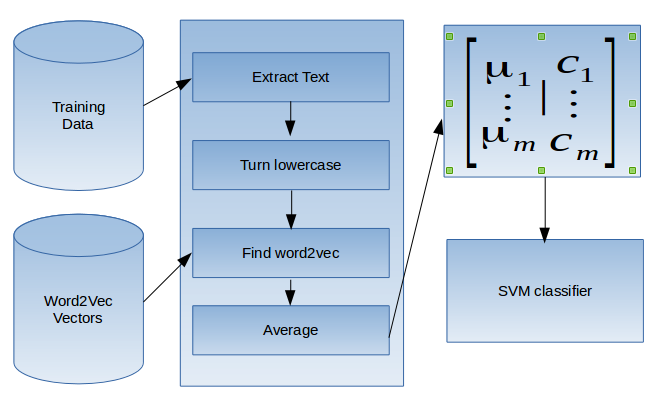
\includegraphics[width=2.5in]{System.png}
\caption{Overview of the system}
\label{System}
\end{figure}

\begin{figure}
\centering

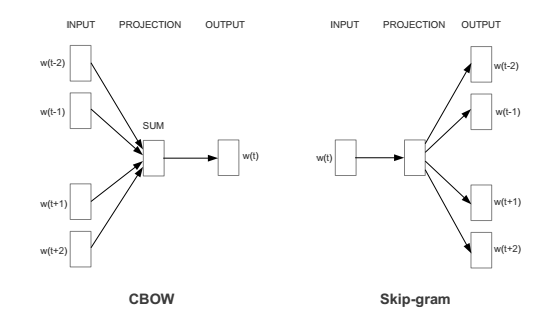
\includegraphics[width=2.5in]{sentiment_01_large.png}
\caption{Diagram for word2vec implementations}
\label{SkipCBOW}
\end{figure}


\begin{figure}
\centering
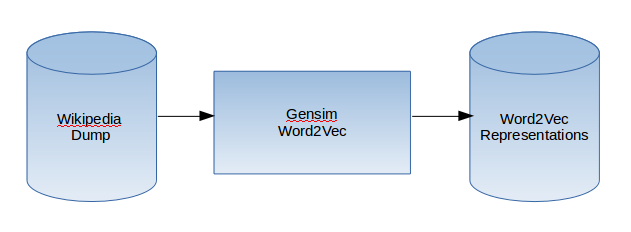
\includegraphics[width=2.5in]{Word2Vec.png}
\caption{Overview of word2vec flow.}
\label{W2vFlow}

\end{figure}


\subsection{Training and Evaluation}
After obtaining word2vec representations for each word as illustrated in figure~\ref{W2vFlow}, each xml document of one twitter user is converted into word2vec representations. To do this, the texts were first extracted from the file. Then it was converted to lower case. After the conversion, the words are checked against the dictionary of all the words that have word2vec representations. If the words exists in the dictionary, the vector representation is pulled out and accumulated, and later normalized by the number of words that could be found in the dictionary. If the word does not exist in the dictionary, a zero vector is returned. 

After representing each twitter user, the vectors are then used as features. Support Vector Machines were then trained using those features. Different kernels and parameters were also checked. This includes polynomial kernel and a radial basis function. For the polynomial kernel, the degrees were restricted to 1, 2, and 3. The C parameter was restricted to 0.01, 1, 100. For the radial basis function, the gammas and C parameters were restricted to 0.01, 1, 100.

The performance of the system was evaluated using the accuracy measure and 10 fold cross validation was used. The parameters that gave the highest accuracies were noted and used in the system deployed in the TIRA server. 

\section{Results and Discussion}
The tables~\ref{EnglishAge}-~\ref{DutchAge} give the all the results for English, Spanish, and Dutch on age and gender. Looking at table~\ref{EnglishAge} for age classification in English, the highest accuracy obtained is 44.8\%. The SVM parameter that gave the best classification is the one with the radial basis function kernel with C to be 1 and gamma to be 100 although most of the other values are close. In gender classification however, the highest accuracy obtained was 68.2\% using a polynomial kernel with the degree to be 3 and C to be 100. There is more variety from these results given that the lowest is around 50.0\%.
\begin{table}[!htbp]
\centering
\caption{Age Classification Results for English}
\label{EnglishAge}
\setlength{\tabcolsep}{0.5em}
{\renewcommand{\arraystretch}{1.2}%
\begin{tabular}{cccccccc}
\toprule
     & \multicolumn{3}{c}{poly}   &  & \multicolumn{3}{c}{rbf}        \\
     & \multicolumn{3}{c}{degree} &  & \multicolumn{3}{c}{gamma}      \\
    & 1       & 2       & 3      &  & 0.01  & 1     & 100            \\
\midrule
C=0.01 & 0.418   & 0.416   & 0.416  &  & 0.414 & 0.414 & 0.414          \\
C=1    & 0.418   & 0.416   & 0.416  &  & 0.414 & 0.418 & \textbf{0.448} \\
C=100  & 0.418   & 0.423   & 0.393  &  & 0.416 & 0.409 & 0.426         \\
\bottomrule 
\end{tabular}
}
\end{table}

\begin{table}[!htbp]
\centering
\caption{Gender Classification Results for English}
\label{EnglishGender}
\setlength{\tabcolsep}{0.5em}
{\renewcommand{\arraystretch}{1.2}%
\begin{tabular}{cccccccc}
\toprule
     & \multicolumn{3}{c}{poly}       &  & \multicolumn{3}{c}{rbf}   \\
     & \multicolumn{3}{c}{degree}     &  & \multicolumn{3}{c}{gamma} \\
    & 1     & 2     & 3              &  & 0.01    & 1       & 100   \\
\midrule
C=0.01 & 0.534 & 0.495 & 0.495          &  & 0.498   & 0.500   & 0.512 \\
C=1    & 0.534 & 0.561 & 0.579          &  & 0.498   & 0.563   & 0.643 \\
C=100  & 0.534 & 0.677 & \textbf{0.682} &  & 0.548   & 0.672   & 0.643 \\
\bottomrule
\end{tabular}
}
\end{table}

The results for Spanish tweets are given below. In table~\ref{SpanishAge}, the highest accuracy for age classification is 51.3\%. This is given by a classifier with a radial basis function kernel with gamma to be 1 and C to be 100. In table~\ref{SpanishGender}, the highest accuracy for gender classification is 67.1\%. This was given by the classifier that used a radial basis function kernel with gamma to be 1 and C to be 100. 
\begin{table}[!htbp]
\centering
\caption{Age Classification Results for Spanish}
\label{SpanishAge}
\setlength{\tabcolsep}{0.5em}
{\renewcommand{\arraystretch}{1.2}%
\begin{tabular}{cccccccc}
\toprule
     & \multicolumn{3}{c}{poly}   &  & \multicolumn{3}{c}{rbf}        \\
     & \multicolumn{3}{c}{degree} &  & \multicolumn{3}{c}{gamma}      \\
    & 1       & 2       & 3      &  & 0.01  & 1              & 100   \\
\midrule
C=0.01 & 0.506   & 0.506   & 0.506  &  & 0.506 & 0.506          & 0.506 \\
C=1    & 0.506   & 0.511   & 0.511  &  & 0.506 & 0.506          & 0.496 \\
C=100  & 0.506   & 0.513   & 0.415  &  & 0.506 & \textbf{0.513} & 0.422 \\
\bottomrule
\end{tabular}
}
\end{table}

\begin{table}[!htbp]
\centering
\caption{Gender Classification Results for Spanish}
\label{SpanishGender}
\setlength{\tabcolsep}{0.5em}
{\renewcommand{\arraystretch}{1.2}%
\begin{tabular}{cccccccc}
\toprule
     & \multicolumn{3}{c}{poly}   &  & \multicolumn{3}{c}{rbf}        \\
     & \multicolumn{3}{c}{degree} &  & \multicolumn{3}{c}{gamma}      \\
    & 1       & 2       & 3      &  & 0.01  & 1              & 100   \\
\midrule
C=0.01 & 0.504   & 0.504   & 0.504  &  & 0.504 & 0.557          & 0.565 \\
C=1    & 0.504   & 0.546   & 0.577  &  & 0.504 & 0.573          & 0.638 \\
C=100  & 0.504   & 0.663   & 0.654  &  & 0.568 & \textbf{0.671} & 0.621 \\
\bottomrule
\end{tabular}
}
\end{table}

Dutch gave the highest accuracy of 71.9\% using an SVM with a radial basis function with a gamma of 1 and C of 100. This is further illustrated in table~\ref{DutchAge}. 
\begin{table}[!htbp]
\centering
\caption{Age Classification Results for Dutch}
\label{DutchAge}
\setlength{\tabcolsep}{0.5em}
{\renewcommand{\arraystretch}{1.2}%
\begin{tabular}{cccccccc}
\toprule
     & \multicolumn{3}{c}{poly}   &  & \multicolumn{3}{c}{rbf}   \\
     & \multicolumn{3}{c}{degree} &  & \multicolumn{3}{c}{gamma} \\
    & 1       & 2       & 3      &  & 0.01    & 1       & 100   \\
\midrule
C=0.01 & 0.547   & 0.513   & 0.513  &  & 0.516   & 0.589   & 0.654 \\
C=1    & 0.542   & 0.641   & 0.649  &  & 0.516   & 0.644   & 0.717 \\
C=100  & 0.539   & 0.719   & 0.685  &  & 0.646   & \textbf{0.719}   & 0.658 \\
\bottomrule
\end{tabular}
}
\end{table}

Finally, we also add the last table~\ref{PANResults} which shows the results given by PAN after using the classifier on a different corpus type. We can see that there is a drop in accuracy between the one tested on tweets and the one on unknown corpus type. For English age classification, we started with 44.8\% which dropped to 35.9\%. 62.8\%

For Spanish age classification, we started with 51.3\% which dropped to 48.2\%, which doesnt seem to be too drastic. For Spanish gender classification, we started with 67.1\% but dropped to 58.9\%. Finally for Dutch, we started with 71.9\% and dropped to 56.8\%.
\begin{table}[!htbp]
\centering
\caption{PAN Results}
\label{PANResults}
\setlength{\tabcolsep}{0.5em}
{\renewcommand{\arraystretch}{1.2}%
\begin{tabular}{cccc}
\toprule
        & Age    & Gender & Joint  \\
\midrule
English & 0.3590 & 0.6282 & 0.2179 \\
Spanish & 0.4821 & 0.5893 & 0.3036 \\
Dutch   & 0.5680 &   -     &  -    \\
\bottomrule 
\end{tabular}
}
\end{table}

It should also be noted that the parameters used in the submitted system differs a bit from the system given here. The system submitted has English to use a radial basis function with gamma and C to be 100. For Dutch and Spanish, the kernel is also a radial basis function with gamma to be equal to 1 and C to be 100. The reason for this difference is that the initial results from previous runs gave these values. 




\section{Conclusion}
The conclusion goes here.

\section{Recommendation}



% conference papers do not normally have an appendix


% use section* for acknowledgment
\section*{Acknowledgment}

The authors would like to thank Erasmus Mundus Mobility for Asia. 





% trigger a \newpage just before the given reference
% number - used to balance the columns on the last page
% adjust value as needed - may need to be readjusted if
% the document is modified later
%\IEEEtriggeratref{8}
% The "triggered" command can be changed if desired:
%\IEEEtriggercmd{\enlargethispage{-5in}}

% references section

% can use a bibliography generated by BibTeX as a .bbl file
% BibTeX documentation can be easily obtained at:
% http://mirror.ctan.org/biblio/bibtex/contrib/doc/
% The IEEEtran BibTeX style support page is at:
% http://www.michaelshell.org/tex/ieeetran/bibtex/
%\bibliographystyle{IEEEtran}
% argument is your BibTeX string definitions and bibliography database(s)
%\bibliography{IEEEabrv,../bib/paper}
%
% <OR> manually copy in the resultant .bbl file
% set second argument of \begin to the number of references
% (used to reserve space for the reference number labels box)
%\bibliographystyle{IEEEtran}
\bibliography{citations}{}
\bibliographystyle{plain}
%\begin{thebibliography}{1}
%
%\bibitem{IEEEhowto:kopka}
%H.~Kopka and P.~W. Daly, \emph{A Guide to \LaTeX}, 3rd~ed.\hskip 1em plus
%  0.5em minus 0.4em\relax Harlow, England: Addison-Wesley, 1999.
%
%\end{thebibliography}




% that's all folks
\end{document}


